\chapter{Implementierung einer grafischen Transceiver Applikation}
Ein in GNU Radio implementierte DAB/DAB+ Sender und Empfänger erfüllen funktionstechnisch alle geforderten Anforderungen. Jedoch ist die Benutzerfreundlichkeit sehr eingeschränkt. Beispielsweise muss die Speicheradresse eines sub-channels manuell aus dem Terminal abgelesen werden um sie im MSC Decoder anzugeben. Um die Benutzterfreundlichkeit zu erhöhen und den DAB/DAB+ Transceiver damit zu einer vollwertigen und ansprechenden Applikation werden zu lassen, wird eine Python Applikation mit grafischem Front-End implementiert.
\subsection{Struktur}
Abb.~\ref{fig:class_diagramm} zeigt das Klassendiagramm der Applikation.

\subsubsection{Python main}
Die Python Klasse "DABstep" stellt das Zentrum der Applikation aus Nutzersicht dar. Sie enthält alle Methoden die den Nutzer mit der App interagieren lassen. Dazu gehören zum einen Setter Methoden die beispielsweise den DAB Empfänger starten oder die Lautstärke regeln und zum anderen Getter Methoden die hauptsächlich für die angezeigten Informationen wie zum Beispiel eine Programmliste zuständig sind.

\subsubsection{Graphisches Frontend}
Die graphischen Informationen zum Design der Applikation liegen in einer separaten Klasse, dem sog. Frontend. Es beinhaltet alle Tabs, Widgets, Beschriftungen, usw. und deren Anordnung im Anzeigefenster der Applikation. Für die Implementierung der \ac{GUI} wird die Python Bibliothek PyQt4 verwendet\footnote{Die aktuelle Nachfolgerversion PyQt5 verwendet Python3 was in GNU Radio noch nicht komplett unterstützt ist.} Ein Großteil des Inhaltes dieser Klasse wurde mit dem Programm QtDesigner4 erzeugt.

\subsection{GNU Radio flowgraphs}
Den funktionellen Kern der Applikation bilden die beiden GNU Radio flowgraphs für den Transmitter und den Receiver. Sie enthalten die Definition, Instanzierung und Verbindung der einzelnen C++ Funktionalblöcke und bilden einen vollwertigen Transmitter bzw. Receiver. Im groben Aufbau entsprechen sie den in den vorherigne Kapiteln vorgestellten GNU Radio flographs aus Abb.~\ref{fig:grc_receiver} bzw. Abb.~\ref{fig:transmitter}. Abhängig von den Argumenten der Klasse, werden die Flowgraphs aber individuell instanziert bzw. initialisiert. Zum Beispiel kann je nach Konfiguration des Empfängers eine Binärdatenquelle oder eine Hardwarequelle als IQ Datenquelle dienen. Im Empfänger können ganze Zweige hinzukommen, wenn mehrere Audiostreams parallel gesendet werden.
Die Flowgraphs laufen in einem separaten Thread. Dies verhindert, dass die komplette Applikation eingefroren ist, wenn der Flowgraph zum Beispiel überlastet ist.

\subsubsection{GNU Radio Blocks}
Die grundlegendste Klasse bilden die C++ Funktionalblöcke. Dazu gehören die in Abschn.~\ref{sec:imp_des_transmitters} und~\ref{sec:impl_des_receivers} beschriebenen Blöcke des in diesem Projekt implementierten Moduls gr-dab, sowie einige grundlegenden Blöcke aus anderen GNU Radio Modulen. Manche Blöcke sind aus Gründen der Übersicht zu hierarchischen Python Blöcken zusammengefasst.
\todo{beschreibe schwerpunkte der blöcke und vor allem ,dass in DABStep möglichst wenig verarbeitung/logik mehr passieren soll}


\begin{figure}[h]
\label{fig:class_diagramm}
\begin{center}
\begin{tikzpicture}[node distance=1cm]
\tikzstyle{class_python}=[
    rectangle,
    rounded corners,
    draw=black,
    %text centered,
    anchor=north,
    text=black,
    text width=4cm]
\tikzstyle{class}=[
    rectangle,
    draw=black,
    %text centered,
    anchor=north,
    text=black,
    text width=4cm]

\node (dabstep) [class_python ,anchor = north, rectangle split, rectangle split parts=3]
    {
        \textbf{\centerline{DABstep}}
        \nodepart{second}-Frontend
        \nodepart{third}+show frontend()\newline+init transmitter()\newline +init receiver()\newline +play audio()\newline +set volume()\newline +get service info()\newline\centerline{...}
    };
\node (Frontend) [class_python, rectangle split, rectangle split parts=2, left =1.0cm of dabstep.north west, anchor = north east] 
    {
        \textbf{\centerline{Frontend}}
        \nodepart{second}-window\newline -tabs\newline -widgets\newline \centerline{...}
    };
\node (lookup tables) [class_python, rectangle split, rectangle split parts=2, right =1.0cm of dabstep.north east, anchor = north west]
    {
        \textbf{\centerline{lookup tables}}
    };
\node (usrp_tx) [class_python, rectangle split, rectangle split parts=3, below left= 1cm and 1cm of dabstep.south]
    {
        \textbf{\centerline{Transmitter}}
        \nodepart{second}-DAB Modus\newline -Frequenz\newline -MCI \& SI\newline -Audioquellen\newline -Ausgabegerät
        \nodepart{third}+run()\newline +set Volume()\newline\centerline{...}
    };
\node (usrp_rx) [class_python, rectangle split, rectangle split parts=3, below right= 1cm and 1cm of dabstep.south]
    {
        \textbf{\centerline{Receiver}}
        \nodepart{second}-DAB Modus\newline -Frequenz\newline -MCI eines Kanals\newline -Quelle (USRP/Datei)
        \nodepart{third}+run()\newline +get MCI()\newline +get SI()\newline +get SNR()\newline +set Volume()\newline\centerline{...}
    };
\node (fib_sink) [class, rectangle split, rectangle split parts=3, text width=3cm, below= of usrp_rx.south, anchor=north west]
    {
        \textbf{\centerline{FIB Senke}}
        \nodepart{third}+get MCI()\newline +get SI() \newline +get CRC passed()
    };
\node (dots3) [left=0.5cm of fib_sink]
    {
        $\cdots$
    };
\node (fic_encode) [class_python, rectangle split, rectangle split parts=2, text width=3cm, below= of usrp_tx]
    {
        \textbf{\centerline{FIC Encoder}}
        \nodepart{second}-DAB Modus
    };
\node (dots1) [right=0.5cm of fic_encode]
    {
        $\cdots$
    };
\node (fib_source) [class, rectangle split, rectangle split parts=2, text width=3cm, left= of fic_encode.north west, anchor = north east]
    {
        \textbf{\centerline{FIB Quelle}}
        \nodepart{second}-DAB Modus\newline -MCI \& SI\newline -DAB oder DAB+
    };
\node (xor) [class, rectangle split, rectangle split parts=2, text width=1.0cm, below= of fic_encode]
    {
        \textbf{\centerline{XOR}}
    };
\node (vector_source) [class, rectangle split, rectangle split parts=2, text width=3cm, below= 0.5cm of xor]
    {
        \textbf{\centerline{Vector Quelle}}
        \nodepart{second}-PRBS Sequenz
    };
\node (dots2) [right=0.5cm of vector_source]
    {
        $\cdots$
    };
\node (crc) [class, rectangle split, rectangle split parts=2, text width=3cm, left= 0.5cm of vector_source.north west, anchor = north east]
    {
        \textbf{\centerline{CRC}}
        \nodepart{second}-FIB Länge\newline -Gen. Polynom\newline -Initalstatus
    };
    
% arrows
\path [line] (Frontend.east) -- (dabstep.west|-Frontend);
\path [line] (lookup tables.west) -- (dabstep.east|-lookup tables);
\path [line] (dabstep.south) |- (usrp_tx.two east);
\path [line] (dabstep.south) |- (usrp_rx.two west);
\path [line] (usrp_rx.north) |- (dabstep.three east);
\path [line] (fib_source.north) -- ($(fib_source.north)+(0.0,0.5)$) -| (usrp_tx.240);
\path [line] (fib_sink.north) -- (usrp_rx.south-|fib_sink.north);
\path [line] (fic_encode.north) -- (usrp_tx.south);
\path [line] (xor.north) -- (fic_encode.south);
\path [line] (crc.north) -- ($(crc.north)+(0.0,0.5)$) -| (fic_encode.210);
\path [line] (vector_source.30) -- (fic_encode.south-|vector_source.30);
\path [line, dotted] (dots1) |- ($(usrp_tx.300)+(0.0,-0.5)$) -- (usrp_tx.300);
\path [line, dotted] (dots3) -- (usrp_rx.south-|dots3);
\path [line, dotted] (dots2) |- ($(fic_encode.south east)+(0.0,-0.5)$) -| (fic_encode.340);

\end{tikzpicture}
\end{center}
\caption{Klassendiagramm der DAB/DAB+ Transceiver Applikation}
\end{figure}

\subsection{Datenfluss}
Ein Großteil des Datenflusses geschieht in den C++ Blöcken, die große Mengen an komplexen IQ Samples oder Bits mit hohen Raten verarbeiten müssen und diese über Ringbuffer an den jeweils nächsten Block weitergeben. Zusätzlich müssen aber auch Daten, wie zum Beispiel die MCI und SI, von den Datenverarbeitungsblöcken zur Benutzeroberfläche transportierte werden um dort in einer strukturierten und für Menschen gut lesbaren Art dargestellt zu werden. Bei diesem Datenstrom fallen geringe Datenmengen an und der Fokus liegt auf einer guten Strukturierung und Charakterisierung der Daten.
Eine geeignete Datenstruktur muss daher folgenden Anforderungen erfüllen:
\begin{itemize}
\item Unterstützung verschiedener Datentypen (string für Sendernamen, integer für Adressierungen, boolean für Bitschalter)
\item Flexible Struktur in:
\begin{itemize}
\item Anzahl der Attribute (das Kanalinfo FIB enthält beispielsweise 5 Attribute, währende das Sendenamen FIB nur 2 Attribute beinhaltet)
\item Anzahl der Elemente (a priori ist nicht bekannt, wie viele Sender im empfangenen Ensemble enthalten sind, bzw. wie viel zusätzliche SI ausgestrahlt wird)
\end{itemize}
\item Gute Lesbarkeit für Menschen
\end{itemize}
Das Format \ac{JSON} erfüllt diese Eigenschaften hinreichend.
\subsubsection{JSON}
Die grundlegenden Datenstrukturen des JSON Formats sind:
\begin{equation}
\begin{aligned}
object =& \biggl\{string : value,\;string : value,\; ...\biggl\} \\
array =& \biggl[value, \;value, \;...\biggl] \\
\text{mit} \; value \; \in& \; \{string,\; number,\; object,\; array,\; true,\; false,\; null\}
\end{aligned}
\end{equation}
Eine für die beschriebenen Anforderungen vorteilhafte Kombination von JSON Strukturen ist in Gl.~\ref{eq:json_example} beispielhaft für ein FIB mit Kanalinformationen dargestellt.
\begin{equation}
\label{eq:json_example}
\begin{aligned}
FIB = \biggl[
& \; \biggl \{ \text{\dq} ID \text{\dq} :4, \text{\dq} address \text{\dq} : 54, \text{\dq} size \text{\dq} : 84, \text{\dq} protection \text{\dq} : 2 \biggl \} \\
& \; \biggl\{\text{\dq}ID\text{\dq}:3,\text{\dq}address\text{\dq}:234,\text{\dq}size\text{\dq}:96,\text{\dq}protection\text{\dq}:3\biggl\} \\
& \; \biggl\{\text{\dq}ID\text{\dq}:2,\text{\dq}address\text{\dq}:54,\text{\dq}size\text{\dq}:54,\text{\dq}protection\text{\dq}:1\biggl\} \biggl]
\end{aligned}
\end{equation}
Das Array liefert die flexible Anzahl an Elementen und das Objekt bietet eine variable Anzahl an Attributen. Die Daten sind gut lesbar und werden genau in dieser Form als String in den jeweiligen Blöcken (eine Vielzahl davon in der FIC Senke) generiert. Diese können dann von der Receiver Klasse über eine get-Funktion abgefrage werden und an die Klasse DABstep weitergeleitet werden, wo sie an entsprechender Stelle angezeigt werden. Das Lesen der Daten in DABstep gestaltet sich besonders intuitiv, da ein JSON Array als Python Array und ein JSON Objekt als Python Dictionary interpretiert werden kann.

\subsection{Graphischer Aufbau}
Neben der Funktionalität steht bei der graphischen Applikation DABstep auch die Benutzerfreundlichkeit im Mittelpunkt. Die Applikation soll auch von Laien intuitiv bedienbar sein und übersichtlich bleiben. Das Programm ist in Empfänger und Sender aufgeteilt die jeweils über zwei Tabs erreichbar sind. Abb.~\ref{fig:GUI_receiver} zeigt die Empfangsseite.
\begin{figure}[h]
\centering
  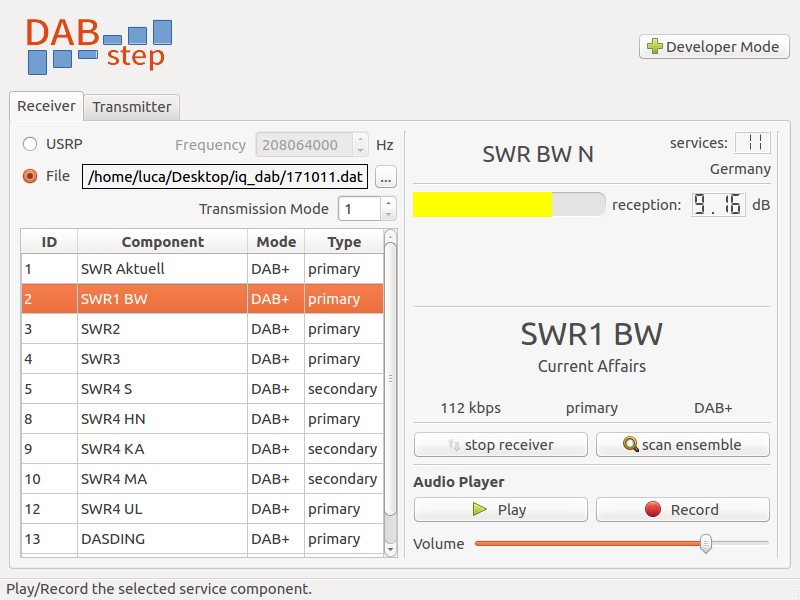
\includegraphics[width=\textwidth]{figures/GUI_receiver.png}
	\caption{DABstep im Empfangsmodus}
	\label{fig:GUI_receiver}
\end{figure}
Die räumliche Aufteilung entspricht in etwa dem Ablauf einer Empfangssituation:
\begin{enumerate}
\item Initiale Einstellungen: Wahl der Quelle und des DAB Modus.
\item Senderliste: Anzeige und Auswahlfeld der DAB Sender.
\item Infos: Anzeige von zusätzlichen Informationen über das Empfangene DAB Ensemble.
\item Audio: Kontrolle über die abgespielte Musik.
\end{enumerate}
Während die Empfangsseite hauptsächlich Informationen anzeigt, liegt der Schwerpunkt bei der Senderseite auf dem Schreiben von Informationen für das zu Sendende DAB Ensemble. Um die Bedienungsfreundlichkeit zu bewahren wurde die Aufteilung im Sender von der funktionalen Aufteilung dem Empfänger nachemfunden. Abb.~\ref{fig:GUI_transmitter} zeigt die GUI im Sendemodus.

\begin{figure}[h]
\centering
  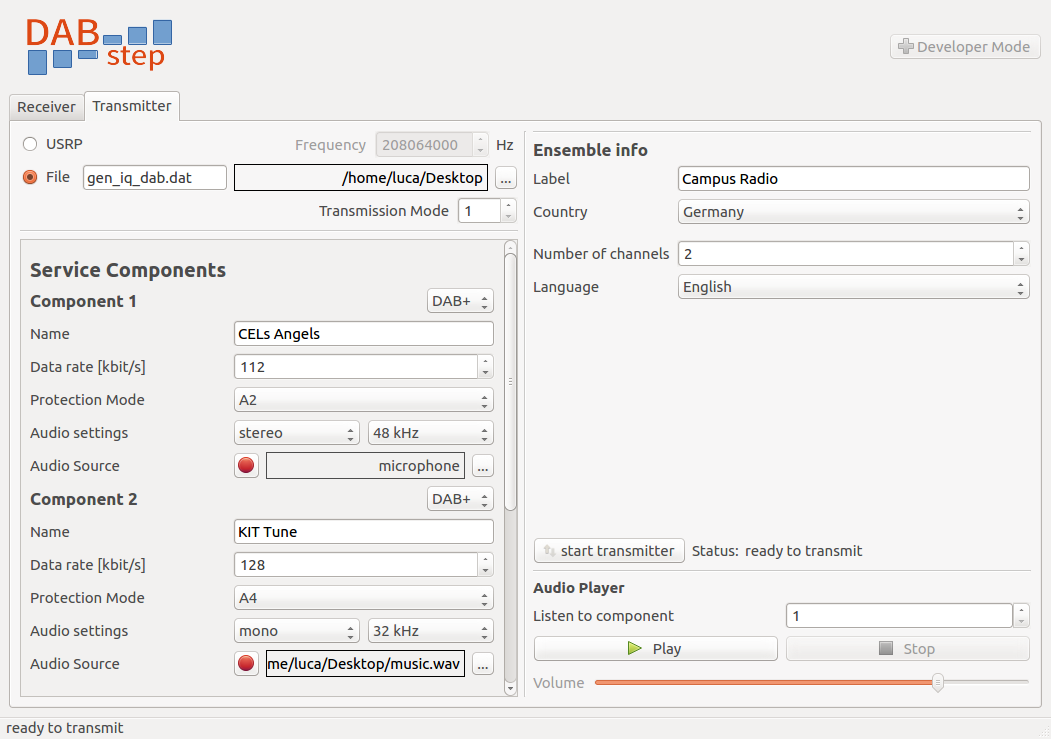
\includegraphics[width=\textwidth]{figures/GUI_transmitter.png}
	\caption{DABstep im Sendemodus}
	\label{fig:GUI_transmitter}
\end{figure}

Durch erhöhen der Anzahl der Kanäle wird die linke Spalte automatisch um eine Komponente ergänzt.

\subsubsection{Entwicklermodus}
Ein zusätzliches Feature stellt der Entwickler-Modus dar, der in der Empfängerseite über das \dq + \dq Symbol in der oberen rechten Ecke erreichbar ist. Dieser erweitert die GUI um einige technische Anzeigen (siehe Abb.~\ref{fig}. 

\begin{figure}[h]
\centering
  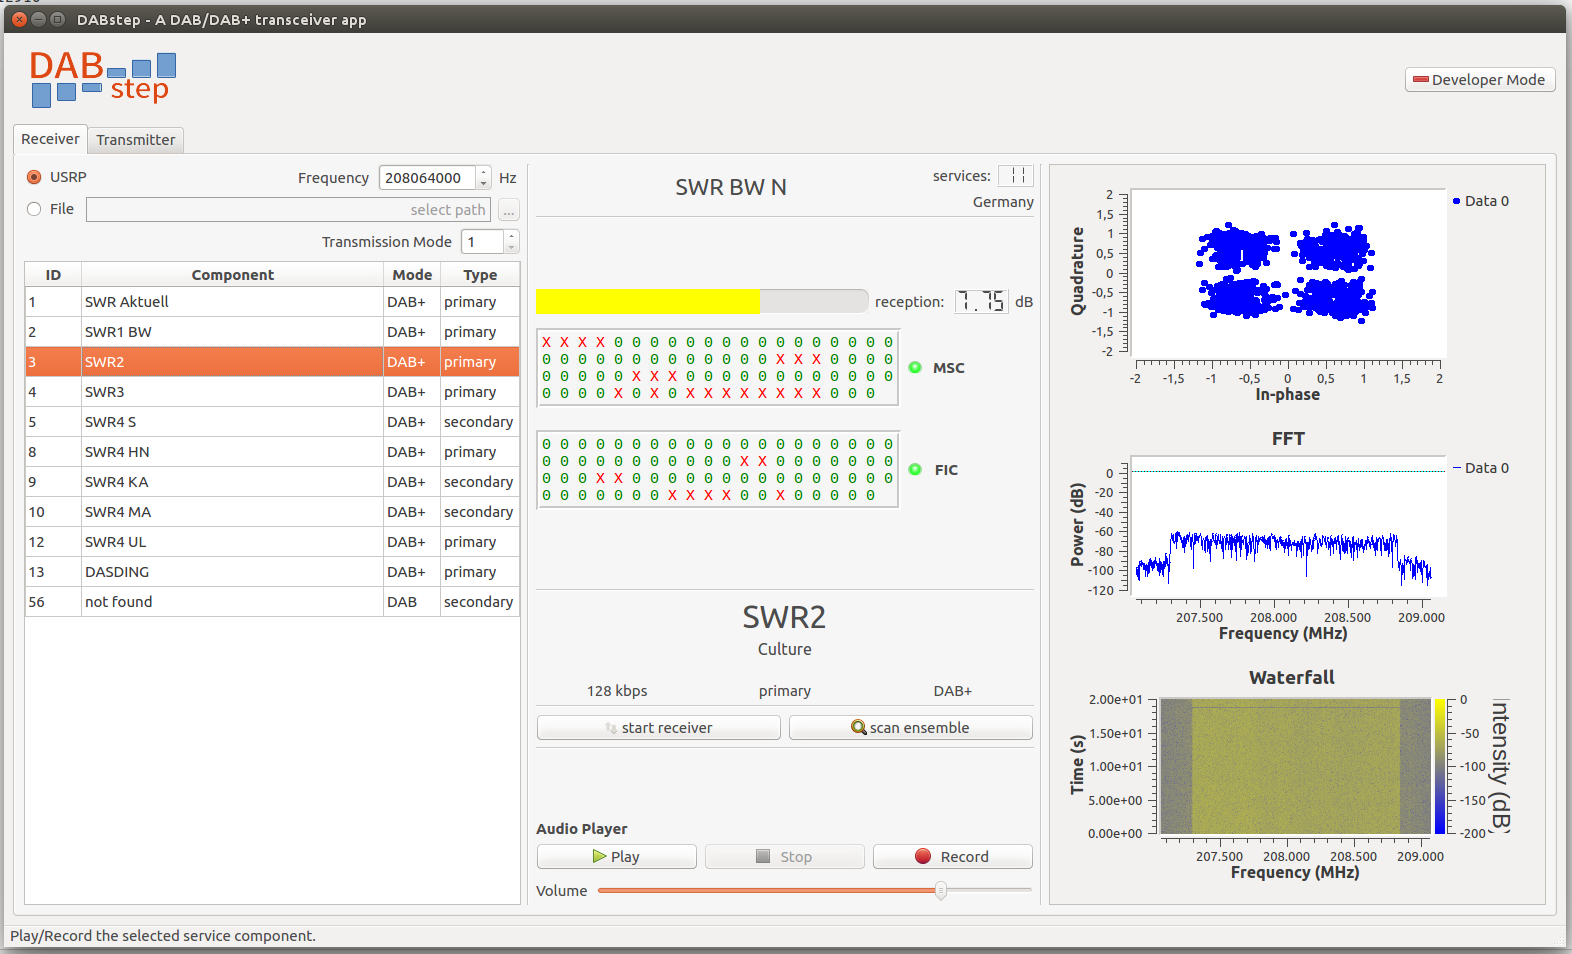
\includegraphics[width=\textwidth]{figures/GUI_dev_mode.png}
	\caption{DABstep im Entwicklermodus}
	\label{fig:GUI_dev_mode}
\end{figure}

Eine Anzeige für die Fehlerrate, getrennt für FIC und MSC, stellt das Ergebnis des CRC checks der FIBs bzw. des Firecode Checks für die Audio Frames dar. Die rechte Spalte ergänzt die GUI um ein Konstellationsdiagramm, eine FFT Anzeige und einen Wasserfall Plot. Die drei Widgets wurden dabei aus dem GNU Radio Modul gr-qtgui übernommen, in den Flowgraph eingebaut und beim Öffnen des Entwicklermodus an die GUI als Objekte übergeben.